\section{Introduction}

\begin{figure}
	\centering
	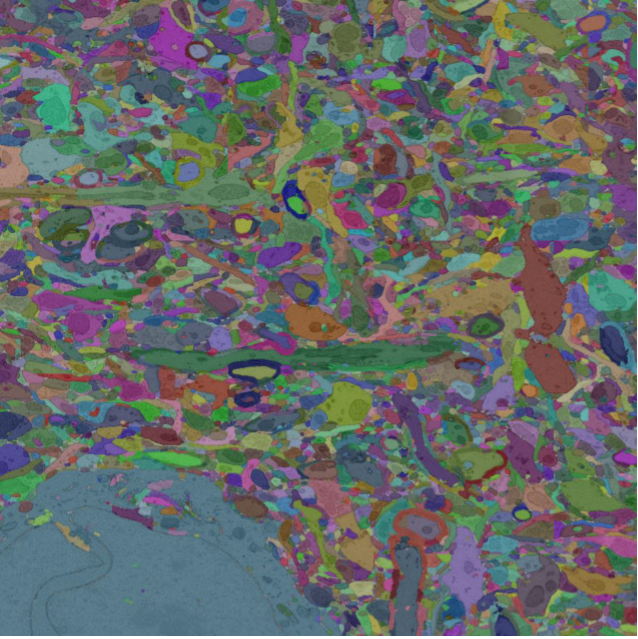
\includegraphics[width=0.42\linewidth]{./figures/intro-slice.png}
	\hspace{0.085\linewidth}
	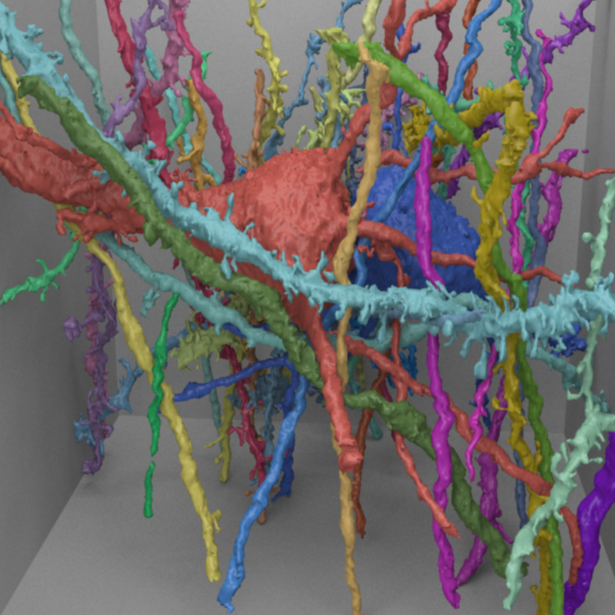
\includegraphics[width=0.42\linewidth]{./figures/intro-cube.png}
\end{figure}

The field of connectomics concerns the wiring diagram of the brain at nanometer resolutions. 
Recent advancements in image acquisition using serial-section electron microscopy (ssEM) has allowed neuroscientists to produce a terabyte of electron micrscopy (EM) image data every hour~\cite{hildebrand2017whole}.
It is not feasible for domain experts to manually segment the vast amount of 3-D image data to model an entire brain.
Neuroscientists believe that reconstructing an entire mammilian brain at fine resolution will enable new insights into the workings of the brain~\cite{kasthuri2015saturated}. 
These observations will allow for new advancements in neuromedicine and artificial intelligence (CITE). 

A significant amount of research focuses on automatic reconstruction of the neurons in these EM images because of the scope and importance of the problem. 
Several of these algorithms attempt to extract complete neurons through the 3-D volumes using only the raw image data as input.
Oftentimes, convolutional neural networks predict membrane probabilities or affinities between voxels and apply simple thresholds to agglomerate the voxels into clusters~\cite{lee2015recursive,ronneberger2015u}.
These \textit{per-voxel} algorithms produce useful outputs but currently fall short of complete reconstructions with sufficient accuracy. 

Researches currently address the failures of the per-voxel algorithms by training random-forest classifiers to agglomerate an oversegmentation of voxels~\cite{nunez2014graph} (CITE NEUROPROOF). 
These classifiers take the output of the per-voxel algorithms as input and generate high-level statistics such as affinity distributions between pixel regions. 
Presently, these methods use hand-designed features despite the evidence that machine-learned features perform better~\cite{bogovic2013learned}. 
These \textit{per-supervoxel} algorithms outperform the per-voxel algorithms but still do not provide the accuracy needed for large scale reconstruction of the brain.
Additionally, these methods do not fully leverage the wealth of shape information available. 

Here we present a \textit{shape-based} strategy that builds on top of the outputs of per-supervoxel methods. 
Similarly we take as input the output of the per-supervoxel methods. 
However, we focus on the overarching shapes traversing through the label volumes to identify potential merge candidates. 
From these locations we extract machine-learned features and generate a probability that two segments should merge. 
Lastly, we construct a graphical representation of the input label volume and apply a global segmentation algorithm to produce a better reconstruction.
Using graph-based optimization strategies enables us to enforce global constraints that more closely match the underlying biology of the images.